\documentclass[12pt,a4]{article}
% 轉成 PDF 時,產生 hyperlink 的效果
\usepackage[dvips]{hyperref}
\usepackage{type1cm}
\usepackage{fancyvrb}
\usepackage{graphicx}
% 在使用 latex2html 可以處理中文
%\usepackage{cwtex}
\usepackage{CJKutf8} %使用CJK套件
\usepackage{comment}
\usepackage{html}

\hypersetup{%
%  dvipdfmx,% 设定要使用的 driver 为 dvipdfmx
  dvips,% 设定要使用的 driver 为 dvipdfmx
  unicode={true},% 使用 unicode 来编码 PDF 字符串
  pdfstartview={FitH},% 文档初始视图为匹配宽度
  bookmarksnumbered={true},% 书签附上章节编号
  bookmarksopen={true},% 展开书签
  pdfborder={0 0 0},% 链接无框
  pdftitle={freetype2 library},
  pdfauthor={descent},
  pdfsubject={develop tools},
  pdfkeywords={freetype2},
  pdfcreator={ps2pdf},
  pdfproducer={PDF 制作程序},% 这个好像没起作用?
}

%\usepackage{appendix}
%\renewcommand{\appendixpagenam}{附錄}
% 標題頁
% 正文
\begin{document}
\begin{CJK}{UTF8}{cwmu} %開始CJK環境,設定編碼,設定字體
\renewcommand{\abstractname}{摘要}
\renewcommand{\figurename}{圖}
\renewcommand{\contentsname}{目錄}
% 標題頁
\begin{titlepage}
\fontsize{30}{30pt plus.5pt minux.4pt}\selectfont
\noindent
%Document Title:\\[6pt]
使用 Autoconf, Automake, Libtool

\fontsize{14}{20pt plus.5pt minux.4pt}\selectfont
\par\vfill\noindent

Author: descent\\
%文件版本:$Revision$
%文件版本:$Id$

\today


\end{titlepage}

文件版本:$Revision: 1.2 $
\newpage
%\addtocontents{toc}{text}
\tableofcontents
\addcontentsline{toc}{section}{REFERENCE}
\newpage


\begin{abstract}
本文件介紹如何用 freetype 來秀出 truetype font。
\end{abstract}
\newpage
\section{freetype library 的呼叫流程}
版本: freetype 2.1.2\\
FT\_{}Init\_{}FreeType() ; // 初使化 freetype library\\
FT\_{}New\_{}Face(); // 從字型載入 face\\
FT\_{}Set\_{}Char\_{}Size(); // 設定 glyph 的大小\\
FT\_{}Get\_{}Char\_{}Index(); // get glyph index\\
FT\_{}Load\_{}Glyph(); // load a glyph image\\
FT\_{}Render\_{}Glyph(); // convert glyph to bitmap

以上均參考\cite{ftdocs}Freetype 2.0 Tutorial Step 1
\subsection{FT\_{}Init\_{}FreeType()}
這個 function 是用來初使化 freetype library。使用方法如下:\\
\begin{Verbatim}[commandchars=@\[\]]
FT_Library  library;
{
 int error = FT_Init_FreeType( &library );
 if ( error )
 {
  // 處理錯誤。
 }
}
\end{Verbatim}
\subsection{FT\_{}New\_{}Face()}
這個 function 會得到一個 face\footnote{字型有斜體、粗體等分類,這便稱做一個 face。}。一個字型最少有一個 face。
以下若有需要用到 face 的 function 就回傳進一個 face 變數。用法如下:
\begin{Verbatim}[commandchars=@\[\]]
FT_Library  library;
{
 int error = FT_Init_FreeType( &library );
 if ( error )
 {
  // 處理錯誤。
 }
}
FT_Face face; // FT_New_Face() 會將 font face 的內容存在這。
// 0 表示第 0 個 face,一定存在的 face
// face->num_faces 可得到這個字型有多少 face
int error = FT_New_Face( library,"arial.ttf",0,&face );
if ( error == FT_Err_Unknown_File_Format )
{
 // 開啟的字型 freetype 不支援
}
else 
 if ( error )
 {
  // 不能開啟該字型。
 }
\end{Verbatim}
\subsection{FT\_{}Set\_{}Char\_{}Size()}
設定 glyph 的大小。用法如下:
\begin{Verbatim}[commandchars=@\[\]]
// 設定 12 points 的大小
// res_x, res_y is device resolution
FT_Set_Char_Size(face,12*64,12*64,res_x,res_y);
// 另一個設定 glyph 大小的 funtion
// pixel_x,pixel_y 的單位為 pixel
FT_Set_Pixel_Sizes(face, pixel_x, pixel_y)
\end{Verbatim}
\subsection{FT\_{}Get\_{}Char\_{}Index()}
當一個 truetype font 被開啟時, freetype 便會選擇 unicode 來做內定的編碼。
選擇編碼的順序是: unicode、 Latin-1、 ASCII。
這個 function 可以從傳入的字集編碼找出此字的 glyph index\footnote{glyph index 就是一個 glyph 在字型中的順序}。

這個 function 會傳回 glyph index, 若傳回 0 表示其 glyph index 不存在。 用法如下:
\begin{Verbatim}[commandchars=@\[\]]
int glyph_index=FT_Get_Char_Index(face,char_code);
\end{Verbatim}
\subsection{FT\_{}Load\_{}Glyph()}
load a glyph image into a glyph slot. 有了 glyph index, 便可以載入一個 glyph image 到 glyh slot\footnote{在 freetype library, glyph slot 會將 glyph image 裝在這裡,不管這個 glyph image 是什麼格式。 ex: outline, or bitmap。}。用法如下:
\begin{Verbatim}[commandchars=@\[\]]
/* load_flags 使用 FT_LOAD_DEFAULT 即可 */
int error = FT_Load_Glyph(face, glyph_index, load_flags );  
// face->glyph->format 可以找出這個 glyph image 是什麼形式的 glyph image。
// 是 bitmap 或是 outline。
// 若 face->glyph->format 的值是 ft_glyph_format_bitmap,
// 便代表這個 glyph image 是以 bitmap 的形式存在 glyph slot。
\end{Verbatim}
\subsection{FT\_{}Render\_{}Glyph()}
若 face-〉glyph-〉format 的值不是  ft\_{}glyph\_{}format\_{}bitmap, 便可以用  
ft\_{}glyph\_{}format\_{}bitamp() 這個 function 來產生一個 bitmap。用法如下:
\begin{Verbatim}[commandchars=@\[\]]
// render_mode 使用 ft_render_mode_normal 即可獲得最好的 render 效果。
// 會產生一個 256 gray levels 的 bitmap, 若用 ft_render_mode_mono
// 會產生 1-bit 的 bitmap。
// face->glyph 是一個 glyph slot。
int error = FT_Render_Glyph(face->glyph, render_mode );
\end{Verbatim}
\newpage
\section{畫出一個 glyph image}
當藉由 FT\_{}Render\_{}Glyph() 產生一個 bitmap 之後,便可以由 face-〉glyph-〉bitmap
來存取這個 bitmap。 face-〉glyph 是一個 glyph slot。而 face-〉glyph-〉bitmap\_{}left,
face-〉glyph-〉bitmap\_{}top 便是 bearingX, bearingY。見圖 1 。
\begin{figure}
\caption{glyph metrics。 圖片來源: freetype 內附文件。}
\begin{center}
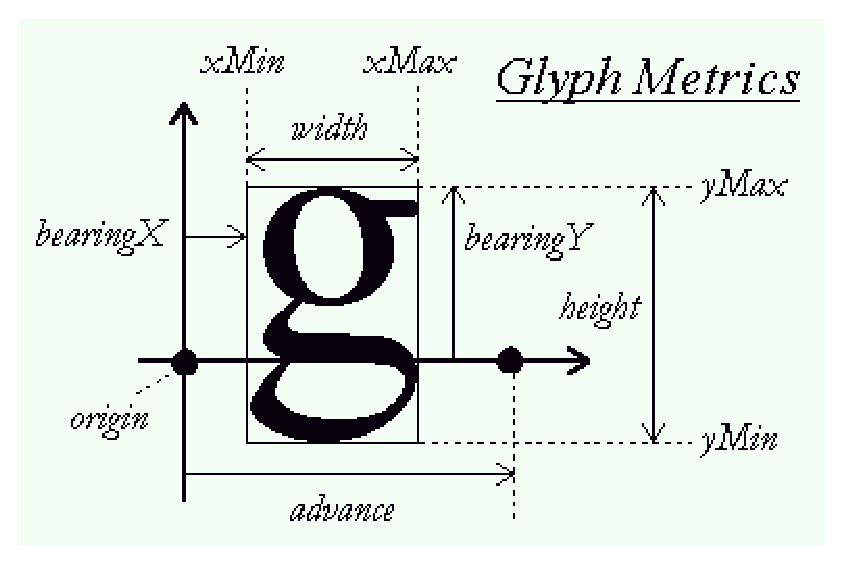
\includegraphics[scale=0.7]{metrics.eps}
\end{center}
\end{figure}
\subsection{用 SVGALIB 來畫出 bitmap}
若使用 SVGALIB library 來畫出一個 bitmap, 可以使用類似下面的 code 來畫出 bitmap。
\begin{Verbatim}[commandchars=@\[\]]
unsigned char *tmp=Bitmap->buffer; // bitmap 的內容
for (int i=0 ; i < Bitmap->rows ; i++) // bitmap 的高
{
 for (int j=0 ; j < Bitmap->width  ; j++) // bitmap 的寬
 {
  if (*tmp)
   // pen_x, pen_y 是要將一個 pixel 畫在螢幕上的座標。
   // gl_setpixelrgb 會畫出一個 pixel
   gl_setpixelrgb(pen_x+j,pen_y+i,*tmp,*tmp,*tmp);
  tmp++;
 }
}
\end{Verbatim}

\subsection{用 QT 來畫出 bitmap}
若使用 QT library 來畫出一個 bitmap, 可以使用類似下面的 code 來畫出 bitmap。
\begin{Verbatim}[commandchars=@\[\]]
QPainter painter;
unsigned char *tmp=Bitmap->buffer; // bitmap 的內容
for (int i=0 ; i < Bitmap->rows ; i++) // bitmap 的高
{
 for (int j=0 ; j < Bitmap->width  ; j++) // bitmap 的寬
 {
  if (*tmp)
  {
   // 將 bitmap 的內容填入 QColor
   QColor color(*tmp,*tmp,*tmp);
   QPen pen(color);
   p.setPen(pen);
   // painter.drawPoint 可以畫出一個 pixel
   painter.drawPoint(pen_x+j,pen_y+i);
  }
  tmp++;
 }
}
\end{Verbatim}
\newpage
\section{字元編碼 (charset)}
由於地方文字的不同, 便有了不同的編碼。 例如 ASCII、Big5、unicode 等等。
以 truetype font 來說都會包含 unicode 編碼。 而 freetype library 的內定值也是選用 
unicode 編碼。
\subsection{將 Big5 編碼轉成 unicode}
若沒有特別轉換, 一般的文字檔就是以 Big5 存成。所以需要將 Big5 轉成 unicode 
來將 unicode 的碼傳給 freetype library。

GLIBC 提供了一系列的函數來提供編碼轉換。 詳情請參閱\cite{glibc}
6.5 Generic Charset Conversion。 主要有三個 function: iconv\_{}open()、 iconv()、 
iconv\_{}close()。

附錄\ref{big52unicode}有一範例。
\subsection{選擇編碼}
freetype library 提供了一個簡便的方法可以選擇編碼。用法如下:
\begin{Verbatim}[commandchars=@\[\]]
// 選定以 unicode 為編碼。
int error=FT_Select_Charmap(face,ft_encoding_unicode);
\end{Verbatim}
以下的程式片段會將 truetype font 內的所有編碼找出來。以 platform id、 encoding id
的形式印出。 查閱 truetype font 的規格文件, 即可找出是何種編碼。
\begin{Verbatim}[commandchars=@\$?]
for (int i=0;i < face->num_charmaps ; ++i)
{
 cout << " platform : " << face->charmaps[i]->platform_id << 
         " encoding : " << face->charmaps[i]->encoding_id << endl;
}

// 這是另一個選用其他編碼的程式片段
// 使用 FT_Set_CharMap function
FT_CharMap  found = 0;
FT_CharMap  charmap;
int n;

for ( n = 0; n < face->num_charmaps; n++ )
{
 charmap = face->charmaps[n];
 if ( charmap->platform_id == my_platform_id &&
      charmap->encoding_id == my_encoding_id )
 {
  found = charmap;
  break;
 }
}

if ( !found ) { ... }

/* now, select the charmap for the face object */
error = FT_Set_CharMap( face, found );
if ( error ) { ... }
\end{Verbatim}
\newpage
\section{字型的其他特性}
這裡介紹 hinting 和 kerning 兩個字型的特性。
\subsection{hinting}
當在顯示較小的 glyph image 時,會有不清楚的情形發生。而 hinting
就是處理此一問題的技術。 truetype font 有其自己的方式, type 1 也有自己的方式,
並不相同。 hinting 有專利的問題。

另一個處理顯示小 glyph image 的技術是 embedded bitmap。舉例來說: embedded 8 points
的字,若要顯示 8 points 的字時,便直接取出,不透過計算。此種方式效果較好。
\subsection{kerning}
kerning 是字與字之間的距離。 中文字因為是方塊字, 所以大多沒有 kerning。
freetype library 提供 FT\_{}Get\_{}Kerning function
來支援 kerning。用法如下:
\begin{Verbatim}[commandchars=@\$?]
FT_UInt       glyph_index;
FT_Bool       use_kerning;
FT_UInt       previous;

.. initialise library ..
.. create face object ..
.. set character size ..

// FT_HAS_KERNING() 用來檢查此字型有無支援 kerning
use_kerning = FT_HAS_KERNING(face);

FT_Vector delta; // after call FT_Get_Kerning, delta 存放 kerning 的資訊
FT_Get_Kerning(face, previous, glyph_index,ft_kerning_mode_default,&delta );
\end{Verbatim}
\newpage
\section{freetype 的進階用法}
freetype library 提供一些進階的用法,可對字型做特殊的處理。如\ref{rotate}所介紹的功能。
\subsection{\label{rotate}旋轉}
使用 FT\_{}Set\_{}Transform function 可以將 glyph image 旋轉某個角度。
以下程式片段將 glyph image 旋轉 30 度。
\begin{Verbatim}[commandchars=+!?]
 // 透過 FT_Set_Transform,將 glyph image 轉個角度。
 // M_PI 是指數學符號 PI
 // PI = 180 度,所以 M_PI/6 = 30 度
 double angle=M_PI/6; // 講 angle 設為 30 度
 FT_Matrix matrix;
 matrix.xx=(FT_Fixed)(cos(angle)*0x10000);
 matrix.xy=(FT_Fixed)(-sin(angle)*0x10000);
 matrix.yx=(FT_Fixed)(sin(angle)*0x10000);
 matrix.yy=(FT_Fixed)(cos(angle)*0x10000);
 FT_Set_Transform(face,&matrix,0);
\end{Verbatim}

FT\_{}Glyph\_{}Transform function 是另一個可以旋轉 glyph image 的方法。
這個 function 要配合其他的 function 來使用。

當有了一個 face 之後,便可以用 FT\_{}Get\_{}Glyph function 來得到一個 
FT\_{}Glyph。 用法如下:
\begin{Verbatim}[commandchars=+!?]
FT_Glyph glyph;
// face->glyph 的 type 是 FT_GlyphSlot
FT_Get_Glyph(face->glyph,&glyph);
\end{Verbatim}
再來便是將 glyph 當參數傳給 FT\_{}Glyph\_{}Transform functio。 若傳入之前需要將
glyph 複製一份的話, 可以用 FT\_{}Glyph\_Copy function 來將 glyph 複製一份。
用法如下:
\begin{Verbatim}[commandchars=+!?]
FT_Glyph glyph2;
FT_Glyph_Copy(glyph,&glyph2);
\end{Verbatim}
至於 FT\_{}Glyph\_{}Transform 可以這樣用:
\begin{Verbatim}[commandchars=+!?]
 // 透過 FT_Set_Transform,將 glyph image 轉個角度。
 // M_PI 是指數學符號 PI
 // PI = 180 度,所以 M_PI/6 = 30 度
 double angle=M_PI/6; // 講 angle 設為 30 度
 FT_Matrix matrix;
 matrix.xx=(FT_Fixed)(cos(angle)*0x10000);
 matrix.xy=(FT_Fixed)(-sin(angle)*0x10000);
 matrix.yx=(FT_Fixed)(sin(angle)*0x10000);
 matrix.yy=(FT_Fixed)(cos(angle)*0x10000);
 FT_Glyph_Transform(glyph,&matrix,0);
\end{Verbatim}
\newpage
\section{獲得一個 bitmap 的其他方法}
在 freetype 裡還可以用其他方式來獲得一個 bitmap。
\subsection{FT\_{}LOAD\_{}Char}
FT\_{}Load\_{}Char function 可以說等於 FT\_{}Get\_{}Char\_{}Index 加上 
FT\_{}Load\_{}Glyph。它有一個特別的參數 loading mode,
若將 FT\_{}LOAD\_{}RENDER 傳入當 loading mode。 便會得到一個 bitmap。 用法如下:
\begin{Verbatim}[commandchars=+!?]
FT_Load_Char(face,text[n],FT_LOAD_RENDER)
若函式呼叫成功,則 face->glyph->bitmap 就可用來存取該 bitmap
\end{Verbatim}
\subsection{FT\_{}Glyph\_{}To\_{}Bitmap}
FT\_{}Glyph\_{}To\_{}Bitmap 是用一個 FT\_{}Glyph 來產生一個 bitmap。 用法如下:
\begin{Verbatim}[commandchars=+!?]
// 0 表示不做 translate ( 有點像座標轉換 )
// 1 是指 destroy original image
FT_Glyph_To_Bitmap(&glyph,ft_render_mode_default,0,1)
\end{Verbatim}
再來把 glyph typecast ( 型別轉換 ) 成 FT\_{}BitmapGlyph 即可。
(FT\_{}BitmapGlyph)glyph。



\newpage
%\section*{}
\section{References}
% reference 指令
\begin{thebibliography}{99}
\bibitem{freetype}www.freetype.org
\bibitem{ftdocs}ftdocs-2.1.2.tar.bz2 由 freetype 網站所提供。\\
(http://sourceforge.net/project/showfiles.php?group\_{}id=3157)
\bibitem{glibc}The GNU C Library Reference Manual
\end{thebibliography}

\newpage
\section{附錄}
\appendix
%\appendixpage
\section{觀看字型資訊的工具}
\begin{itemize}
\item
gfontview ( http://www.gnu.org/directory/gfontview.html )\\
要有 t1lib(libt1.so.*),才能編譯成功。Type1 (*.pfb)/TTF/TTC 字型,而且可以做放大的功能 (mouse 左、中、右鍵是三段放大的功能)。
\item
pfaedit ( http://pfaedit.sourceforge.net/ )\\ 
這個軟體不僅可以觀看,而且也可以編輯 Type*/TTF/TTC 字型。 
\newpage
\end{itemize}
\section{\label{big52unicode}將 Big5 轉成 unicode 的程式}
\begin{Verbatim}[commandchars=@\^?,numbers=left]
// convert.h
/*
 *
 * $Revision: 1.2 $
 * $Author: descent $
 * $Date: 2002/09/25 03:02:16 $
 * $Id: freetype_t.ctx,v 1.2 2002/09/25 03:02:16 descent Exp $
 * function : use iconv serial function to conver any code to another code.
 *            Now only support to convert to unicode. 
 */

#ifndef CONVERT_H
#define CONVERT_H

#include <iconv.h>
#include <cstdio>
#include <errno.h>
#include <stddef.h>
#include <cstdio>

#include <iostream>
#include <string>
#include <fstream>
#include <vector>

#include <cstring>


namespace DS
{

 class ConvertException
 {
  public:
   const std::string &msg(){return _msg;}
   const int err(){return _errno;}
   ConvertException(int err,const std::string &msg):_msg(msg)
   {
    _errno=err;
   }
  private:
   std::string _msg;
   int _errno;
 };

 class Convert
 {
  public:
   Convert(const std::string &from_code="BIG5",
           const std::string &to_code="UNICODE"):
	   _from_code(from_code),_to_code(to_code)
   {
    _convert_len=0;
    _cd=iconv_open(to_code.c_str(),from_code.c_str());
    if (_cd==(iconv_t)(-1))
    {
     switch (errno)
     {
      case EINVAL:
      {
       throw DS::ConvertException(EINVAL,"EINVAL : conversion from '" + 
                                  _from_code + "' to '" + _to_code + 
				  "' not available");
       break;
      }
      case EMFILE:
      {
       throw DS::ConvertException(EMFILE,"EMFILE : The process already has 
                                  OPEN_MAX file descriptors open.");
       break;
      }
      case ENFILE:
      {
       throw DS::ConvertException(ENFILE,"ENFILE : The system limit of 
                                  open file is reached.");
       break;
      }
      case ENOMEM:
      {
       throw DS::ConvertException(ENOMEM,"ENOMEM : Not enough memory to 
                                  carry out the operation.");
       break;
      }

     } // end switch (errno)
    } // end if (_cd==(iconv_t)(-1))
   } // end Convert()

   const char* conv(const std::string &str)
   {
    char *src=const_cast<char*>(str.c_str());
    size_t len=str.length();
    size_t den_len=4*len;
    size_t nconv;
    char *denstr;
    denstr=new char [den_len] ;
    char *den_ptr=denstr;
     //std::cout << den_len << std::endl;
    nconv=iconv(_cd,&src,&len,&den_ptr,&den_len);
     
    if (nconv==(size_t)(-1))
    {
     switch (errno)
     {
      case EILSEQ :
      {
       throw DS::ConvertException(EILSEQ,"EILSEQ : 
                                  The conversion stopped because of 
				  an invalid byte sequence in the input. 
				  After the call *inbuf points at the first 
				  byte of the invalid byte sequence.");
       break;
      }
      case E2BIG :
      {
       throw DS::ConvertException(E2BIG,"E2BIG : The conversion stopped 
                                  because it ran out of space 
				  in the output buffer.");
       // extend dep_ptr and deln_len
       break;
      }
      case EINVAL :
      {
       throw DS::ConvertException(EINVAL,"EINVAL : 
                                  The conversion stopped because of an 
				  incomplete byte sequence at the end of 
				  the input buffer.");
       break;
      }
      case EBADF :
      {
       throw DS::ConvertException(EBADF,"EBADF : The cd argument is invalid.");
       break;
      }

     } // end switch (errno)

    } // if (nconv==(size_t)(-1))
    _convert_len=den_ptr-denstr;
    _to_char_set=denstr;
    return _to_char_set;
   }

   ~Convert()
   {
    delete [] _to_char_set;
    if (iconv_close(_cd) != 0)
     throw DS::ConvertException(EBADF,"EBADF : 
                                The conversion descriptor is invalid.");
   }
   const size_t get_convert_size() const {return _convert_len;}
  private:
   std::string _from_code,_to_code;
   iconv_t _cd;
   char *_to_char_set;
   size_t _convert_len;
 };

 inline std::vector<ushort> to_unicode(std::string &str)
 {
  DS::Convert conv;
  const char * to_char_set=conv.conv(str);
  const size_t len=conv.get_convert_size();

  std::vector<ushort> unicode;
  std::cout << "len : " << len << std::endl;
  for(int i=2 ; i < len ; i+=2)
  {
   ushort code=0;
   unsigned char hi_byte,lo_byte;
   //ushort hi_byte,lo_byte;
   lo_byte=to_char_set[i];
   hi_byte=to_char_set[i+1];
   code=((hi_byte | 0) << 8 ) | lo_byte;

   unicode.push_back(code);
  }
  return unicode;

 }
} // end namespace DS

#endif

// convert.cpp
#include "convert.h"
\end{Verbatim}
\newpage
\section{範例程式, 使用 SVGALIB 來秀字}
\begin{Verbatim}[commandchars=@\^?,numbers=left]

/*
 * $Author: descent $
 * 程式功能:使用 svgalib 秀出字型。此程式會秀出一個 '泉' 並旋轉 30 度
 */
	
#include <ft2build.h>
#include FT_FREETYPE_H
#include FT_GLYPH_H
#include <iostream>
#include <string>
#include <cstdlib>
#include <cmath>
#include <vga.h>
#include <vgagl.h>

#include "convert.h"

using namespace std;

typedef struct TGLYPH_
{
 FT_UInt glyph_index;
 FT_Glyph image;
}TGlyph,*PGlyph;

const int MAX_GLYPHS=512;

int main(int argc,char **argv)
{
 void my_draw_bitmap(FT_Bitmap *Bitmap,int pen_x,int pen_y);
 FT_Vector vector;
 TGlyph glyphs[MAX_GLYPHS];
 PGlyph glyph=glyphs;
 FT_Library library;
 FT_Face face;
 FT_Error error;
 system("clear");
 string fontpath="/usr/share/fonts/zh_TW/TrueType/bsmi00lp.ttf";
 if (argc > 1)
  fontpath=argv[1];

 error=FT_Init_FreeType(&library);
 if (error!=0)
 {
  cout << "FT_Init_FreeType(&library) error!!" << endl;
  return -1;
 }
 error=FT_New_Face(library,fontpath.c_str(),0,&face); // 從字型載入 face
 if (error==FT_Err_Unknown_File_Format)
 {
  cout << "Don't support this font file" << endl;
  return -1;
 }
 else if (error)
      {
       cout << "The font file cann't be opened!" << endl;
       return -1;
      }
 cout << "face information : " << endl;
 cout << "face number is : " << face->num_faces << endl;
 cout << "face glyphs number is : " << face->num_glyphs << endl;
 cout << "face's sytle name is : " << face->style_name << endl;
 cout << "units per EM : " << face->units_per_EM << endl;
 cout << "num_fixed_sizes : " << face->num_fixed_sizes << endl;
 if (face->charmap==NULL)
  cout << "No charmap is selected" << endl;
 cout << "charmap numbers is : " << face->num_charmaps << endl;
 error=FT_Select_Charmap(face,ft_encoding_unicode);
 if (error)
 {
  cout << "FT_Select_CharMap(face,ft_encoding_unicode) error"  << endl;
  return -1;
 }
 std::string text="泉";
 std::vector<ushort> unicode;
 unicode=DS::to_unicode(text); // 將 '泉' 轉成 unicode
 int glyph_index=FT_Get_Char_Index(face,unicode[0]);
 glyph_index=FT_Get_Char_Index(face,charcode);
 if (glyph_index==0)
 {
  cout << "glyph index not found" << endl;
  return 0;
 }

 error=FT_Set_Char_Size(face,0,10*64,360,360);
 if (error)
 {
  cout << "FT_Set_Pixel_Sizes error" << endl;
  return -1;
 }
 // 將 glyph image 轉個角度,透過 FT_Set_Transform
 FT_Matrix matrix;
 double angle=M_PI/6;
 matrix.xx=(FT_Fixed)(cos(angle)*0x10000);
 matrix.xy=(FT_Fixed)(-sin(angle)*0x10000);
 matrix.yx=(FT_Fixed)(sin(angle)*0x10000);
 matrix.yy=(FT_Fixed)(cos(angle)*0x10000);
 FT_Vector pen;
 pen.x=300*64;
 pen.y=300*64;
 FT_Set_Transform(face,&matrix,&pen);
 
 if (glyph_index!=0)
 {
  FT_Int load_flags=FT_LOAD_DEFAULT;
  error=FT_Load_Glyph(face,glyph_index,load_flags);
  if (error!=0)
  {
   cout << "FT_Load_Glyph(face,glyph_index,load_flags) is fail " << endl;
   cout << "The error number is : " << error << endl;
   return -1;
  }
  if (face->glyph->format!=ft_glyph_format_bitmap)
  {
   cout << "run FT_Render_Glyph" << endl;
   //error=FT_Render_Glyph(face->glyph,ft_render_mode_normal);
   error=FT_Render_Glyph(face->glyph,0);
   if (error)
   {
    cout << "FT_Render_Glyph error " << endl;
    return -1;
   }
  }
 } // end FT_Load_Glyph
 FT_GlyphSlot slot=face->glyph;
 my_draw_bitmap(&slot->bitmap,slot->bitmap_left,slot->bitmap_top);
 
 FT_Done_FreeType(library);

}

void my_draw_bitmap(FT_Bitmap *Bitmap,int pen_x,int pen_y)
{
 cout << "Bitmap rows : " << Bitmap->rows << endl;
 cout << "Bitmap width : " << Bitmap->width << endl;
 cout << "Bitmap pitch : " << Bitmap->pitch << endl;
 if (Bitmap->pixel_mode==ft_pixel_mode_mono)
  cout << "Bitmap pixel mode : mono" << endl;
 if (Bitmap->pixel_mode==ft_pixel_mode_grays)
 {
  cout << "Bitmap pixel mode : grays" << endl;
  cout << "Bitmap grays level : " << Bitmap->num_grays << endl;
 }

 vga_init();
 int vga_mode=G1024x768x16M;
 vga_setmode(vga_mode);
 gl_setcontextvga(vga_mode);
 vga_clear();
 unsigned char *tmp=Bitmap->buffer;
 for (int i=0 ; i < Bitmap->rows ; i++)
 {
  for (int j=0 ; j < Bitmap->width ; j++)
  {
   if (*tmp)
    gl_setpixelrgb(pen_x+j,pen_y+i,*tmp,*tmp,*tmp);
   tmp++;
  }
 }
 vga_getch();

 vga_setmode(TEXT);

}
\end{Verbatim}
\end{CJK}{UTF8}{cwmu}
\end{document}
